\section{Tần suất sử dụng thuật toán hủy, chèn}

Trong phần này, chúng ta sẽ theo dõi trọng số của các thuật toán hủy, chèn qua các vòng lặp. Từ đó ta biết được rằng liệu thuật toán hủy hay chèn có hiệu quả (trọng số cao) hay không hay các thuật toán hủy, chèn đó hiệu quả (hoặc không) vào giai đoạn nào của ALNS.
 
\begin{figure}[H] % places figure environment here   
	\centering % Centers Graphic
	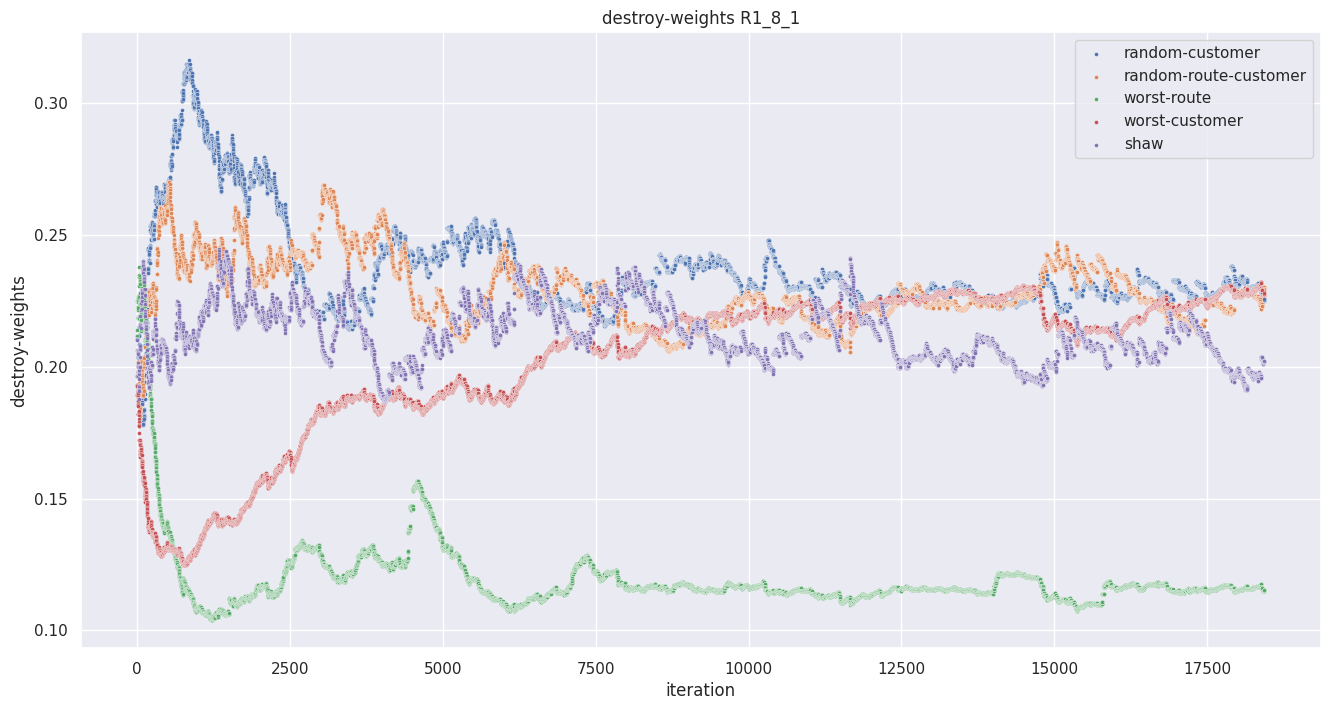
\includegraphics[width=1\textwidth]{figures/destroy_weights_R1_8_1.png}
	% \includesvg[scale=1]{figures/core-object}
	\caption{Trọng số của các thuật toán hủy}
	\label{fig:alg_01}
\end{figure}


\begin{figure}[H] % places figure environment here   
	\centering % Centers Graphic
	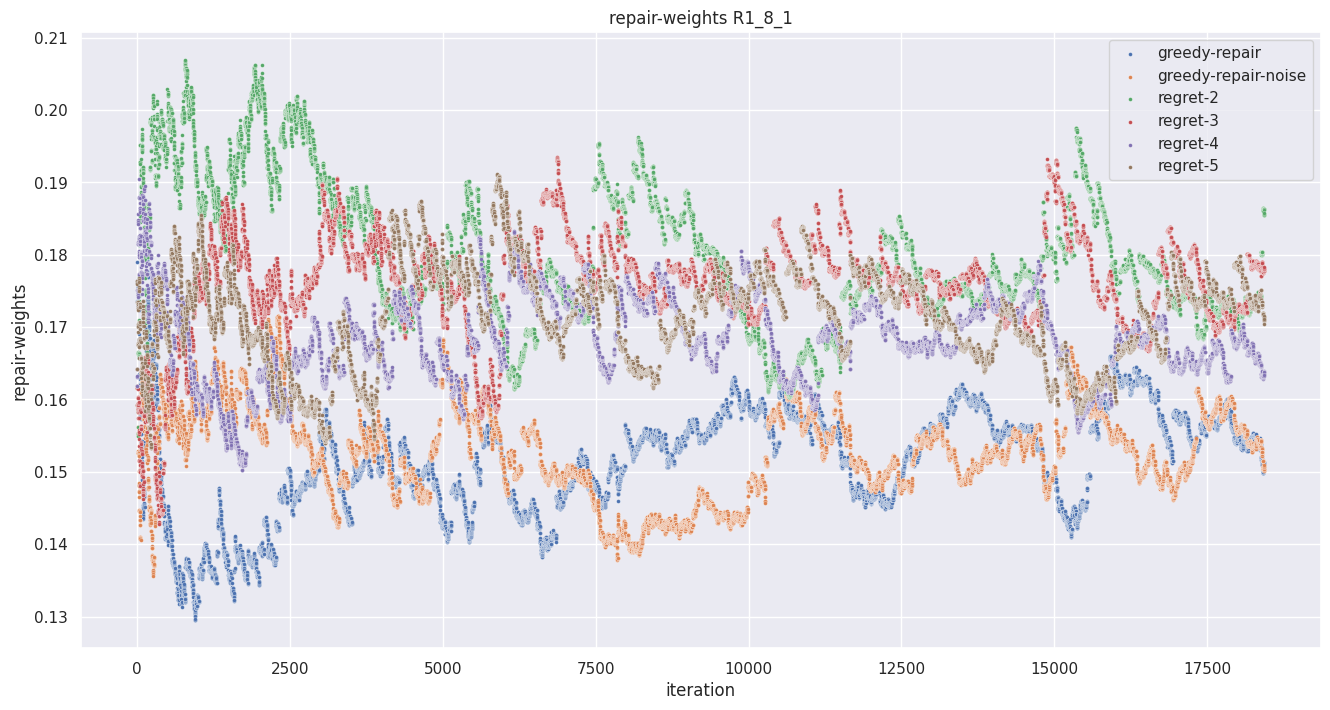
\includegraphics[width=1\textwidth]{figures/repair_weights_R1_8_1.png}
	% \includesvg[scale=1]{figures/core-object}
	\caption{Trọng số của các thuật toán chèn}
	\label{fig:alg_02}
\end{figure}

\subsection*{Thuật toán hủy}
Trong giai đoạn đầu của ALNS, thuật toán \textit{hủy tuyến tệ} được sử dụng nhiều (trọng số cao) nhưng về sau thì tần suất sử dụng lại giảm dần. Không khó hiểu khi ban đầu, các tuyến được sắp xếp chưa thực sự hiệu quả nên ta có thể xóa toàn bộ yêu cầu trong một số tuyến nhất định và chèn vào các tuyến khác. Đến giai đoạn sau của ALNS, khi các tuyến đường đã chứa những yêu cầu quan trọng (nghĩa là rất khó để chèn chúng vào một tuyến đường khác), ta khó có thể xóa cả tuyến đường. Việc thuật toán hủy tuyến được sử dụng nhiều vào giai đoạn đầu của ALNS giúp giảm nhanh số xe được sử dụng. Thực chất, ta cũng chỉ muốn sử dụng hủy tuyến vào giai đoạn đầu của thuật toán. ALNS tự điều chỉnh trọng số của các thuật toán hủy, chèn khiến chúng ta không cần phải thiết lập phức tạp trong khi cài đặt, ví dụ như ta chỉ muốn thuật toán hủy, chèn nhất định được sử dụng trong giai đoạn nào đó trong quá trình chạy ALNS. 

Ngược lại với thuật toán \textit{hủy tuyến tệ}, thuật toán \textit{hủy yêu cầu tệ} cho thấy hiệu quả vào giai đoạn sau của ALNS. Thuật toán \textit{hủy yêu cầu ngẫu nhiên}, \textit{hủy yêu cầu ngẫu nhiên với tuyến} hay thuật toán hủy \textit{Shaw} cho thấy sự "ổn định" khi luôn giữ trọng số cao trong suốt quá trình chạy ALNS.

\subsection*{Thuật toán chèn}
Đối với các thuật toán chèn, ta thấy rõ sự hiệu quả của nhóm các thuật toán \textit{hối tiếc} khi so sánh với nhóm \textit{tham lam} khi trong suốt quá trình chạy, các thuật toán chèn \textit{hối tiếc} luôn giữ trọng số cao. Nói riêng về thuật toán \textit{tham lam}, trong giai đoạn đầu (dưới $2500$ bước lặp), ta thấy rằng việc thêm nhiễu mang lại hiệu quả hơn so với việc chỉ chèn các yêu cầu vào vị trí làm tăng hàm mục tiêu ít nhất. 
